\documentclass[9pt,twocolumn,twoside]{pnas-new}

\usepackage{bm, amsmath, nicefrac}


\templatetype{pnasresearcharticle} % Choose template
\setboolean{displaywatermark}{false}

\usepackage{bm,bbm}
\usepackage{pstricks}

\newcommand{\cW}{\mathcal{W}}
\newcommand{\cM}{\mathcal{M}}
\newcommand{\cR}{\mathcal{R}}
\newcommand{\cX}{\mathcal{X}}
\newcommand{\EE}{\mathbb{E}} \newcommand{\RR}{\mathbb{R}}
\newcommand{\NN}{\mathbb{N}} \newcommand{\ZZ}{{\mathbb{Z}}}
\newcommand{\CC}{{\mathbb{C}}}
\newcommand{\truedata}{\bm{x}}
\newcommand{\weight}{\bm{a}}
\newcommand{\truealloc}{\alloc{\truedata}}
\newcommand{\noisyalloc}{\alloc{\noisydata}}
\newcommand{\noisydata}{\tilde{\bm{x}}}
\newcommand{\norm}[1]{\left\lVert#1\right\rVert}

\newcommand{\diff}[1]{\bm{d}\left(#1\right)}
\newcommand{\col}[1]{\operatorname{col}\left(#1\right)}
\newcommand{\row}[1]{\operatorname{row}\left(#1\right)}
\newcommand{\rank}[1]{\operatorname{rank}\left(#1\right)}
\newcommand{\tr}[1]{\operatorname{tr}\left(#1\right)}
\newcommand{\cov}[1]{\operatorname{Cov}\left(#1\right)}
\newcommand{\lspan}[1]{\operatorname{span}\left(#1\right)}

\newcommand{\bias}[2]{\operatorname{Bias}\left(#1,#2\right)}
\newcommand{\diserr}[2]{\xi\left(#1,#2\right)}
\newcommand{\pr}[1]{\operatorname{Pr}\left(#1\right)}
\newcommand{\var}[1]{\operatorname{Var}\left(#1\right)}
\newcommand{\inner}[2]{\left\langle#1,#2\right\rangle}
\newcommand{\vecangle}[2]{\angle\left(#1,#2\right)}
\newcommand{\err}[1]{\operatorname{Err}\left(#1\right)}
\newcommand{\proj}[2]{\Pi_{#1}\left(#2\right)}
\newcommand{\BB}[2]{B_{#1}\left(#2\right)}
\newcommand{\opt}[1]{\operatorname{Opt}\left(#1\right)}
\newcommand{\relu}[1]{\left(#1\right)_+}
\newcommand{\alloc}[1]{P^F\left(#1\right)}
\newcommand{\blmech}[1]{\cM_{\mathrm{BL}}\left(#1\right)}
\newcommand{\posmech}[1]{\cM_{\mathrm{PoS}}\left(#1\right)}
\newcommand{\andmech}[1]{\cM_{\mathrm{A\&D}}\left(#1\right)}
\newcommand{\pamech}[1]{\cM_{\mathrm{PA}}\left(#1\right)}
\newcommand{\rpmech}[1]{\cM_{\mathrm{RP}}\left(#1\right)}
\newcommand{\talloci}[1]{P^F_{#1}\left(\truedata\right)}
\newcommand{\nalloci}[1]{P^F_{#1}\left(\noisydata\right)}

\newcommand{\unit}{\bm{e}}
\newcommand{\newunit}{\bm{e}'}

\newcommand{\refopt}{\operatorname{Ref}}
\newcommand{\supp}{\operatorname{supp}}
\newcommand{\noise}{\bm{\eta}}
\newcommand{\cop}{B^+}
\newcommand{\radius}{r_m}

\newcommand{\cN}{{\mathcal{N}}}
\newcommand{\cI}{{\mathcal{I}}}
\newcommand{\cJ}{{\mathcal{J}}}
\newcommand{\chat}{\hat{\bm{c}}}
\newcommand{\dhat}{\hat{\bm{d}}}

\newtheorem{definition}{Definition}
\newtheorem{assumption}{Assumption}
\newtheorem{corollary}{Corollary}
\newtheorem{problem*}{Problem}
\newtheorem{property}{Property}
\newtheorem{theorem}{Theorem}
\newtheorem{lemma}{Lemma}
\newtheorem{remark}{Remark}
\newtheorem{proposition}{Proposition}
\newtheorem{claim}{Claim}
\newtheorem{example}{Example}




\begin{document}

	\title{Bias in allocations using differentially private census data: An analysis of the 2020 U.S.~Census}

	% Use letters for affiliations, numbers to show equal authorship (if applicable) and to indicate the corresponding author
	\author[a,c,1]{Author One}
	\author[b,1,2]{Author Two}
	\author[a]{Author Three}

	\affil[a]{Affiliation One}
	\affil[b]{Affiliation Two}
	\affil[c]{Affiliation Three}

	% Please give the surname of the lead author for the running footer
	\leadauthor{Lead author last name}

	% SIGNIFICANCE STATEMENT
	\significancestatement{This research addresses a critical gap in understanding the
relationship between privacy-preserving data release methods,
	particularly differential privacy, and the fairness of consequen-
	tial societal decisions derived from such data. By investigating
	the impacts of differential privacy on resource allocation, this
	study unveils the inherent potential for bias against various
	groups, which could detrimentally affect areas such as educa-
	tional funding, electoral assistance, and public health initiatives.
	In response to these findings, our work proposes guidelines
	to bound unfairness and foster equity, providing a roadmap for
	future applications of differential privacy in data-driven decision
	making. The insights gleaned from this study have implications
	not only for the application of privacy-preserving techniques,
	but also for broader conversations around data privacy, fairness,
	and social equity}


	% Please include corresponding author, author contribution and author declaration information
	\authorcontributions{Please provide details of author contributions here.}
	\authordeclaration{Please declare any competing interests here.}
	\equalauthors{\textsuperscript{1}A.O.(Author One) contributed equally to this work with A.T. (Author Two) (remove if not applicable).}
	\correspondingauthor{\textsuperscript{2}To whom correspondence should be addressed. E-mail: author.two\@email.com}

% At least three keywords are required at submission. Please provide three to five keywords, separated by the pipe symbol.
	\keywords{Differential Privacy $|$ Fairness $|$ Resource Allocation $|$ Census}

	% ABSTRACT
	\begin{abstract}
	The decennial census is a primary source of data for the US government to make critical decisions. For example,
	132 programs used Census Bureau data to distribute more than \$675 billion in funds during fiscal year
	2015. In order to ensure the published census data does not reveal individual information, the Census Bureau adopts
	the differential privacy (DP) technique. In particular, in 2020, the Census Bureau implemented the Top Down
	algorithm which release statistical data from top (nation) to bottom hierarchical level (block). However, it was
	recently observed that the DP outcomes can introduce biased outcomes, especially for minority groups. In this paper,
	we analyze the reasons for these disproportionate impacts and proposes guidelines to mitigate these effects. We
	focus on two aspects that can produce the fair outcomes: (1) shape of allocation function and (2) impact of
	post-processing steps.
\end{abstract}

	\dates{This manuscript was compiled on \today}
	\doi{\url{www.pnas.org/cgi/doi/10.1073/pnas.XXXXXXXXXX}}


	\maketitle
	\thispagestyle{firststyle}
	\ifthenelse{\boolean{shortarticle}}{\ifthenelse{\boolean{singlecolumn}}{\abscontentformatted}{\abscontent}}{}
	\firstpage[20]{5}

	\section*{Introduction}

Agencies, such as the U.S.~Census Bureau, release data sets and
statistics about groups of individuals that are then used as inputs to
a number critical decision processes. For example, the census data is
used to decide whether a jurisdiction must provide language assistance
during elections, Title I fund allocation in education \cite{pujol:20}
and to establish national level COVID-19 vaccination distribution plans
for states and jurisdictions \cite{covid}.
The resulting decisions can have significant societal, economic, and medical
consequences for participating individuals.

In many cases, the released data
contain sensitive information and their privacy is strictly regulated.
For example, in the U.S., the census data is regulated under Title 13
\cite{title13}, which requires that no individual be identified from
any data release by the Census Bureau. In Europe, data release are
regulated according to the \emph{General Data Protection Regulation}
\cite{GDPR}, which addresses the control and transfer of personal data.

Statistical agencies thus release \emph{privacy-preserving} data and
statistics that conform to privacy and confidentiality requirements.
In the U.S., a small number of decisions, such as congressional
apportionment, are taken using unprotected true values, but the vast
majority of decisions rely on privacy-preserving data. Of particular
interest are resource allocation decisions relying on the U.S.~Census
Bureau data, since the bureau will release several privacy-preserving
data products using the framework of \emph{Differential Privacy} \cite{abowd2018us}
for their 2020 release.

In particular, in 2020 the Census Bureau implemented a new privacy preserving framework to release privately hierarchical
statistical data, the Top Down algorithm. The algorithms works by firstly splitting the given privacy budget $\epsilon$ to six
hierarchical levels (nation, state, county, tract, block, group—block). Then in the second step, a post-processing step
is applied to make sure the noisy counts are consistent, e.g., the counts should be non-negative.
However, \cite{pujol:20} empirically showed that differential privacy may have a disparate impact on several resource
allocation problems. The noise introduced by the privacy mechanism may result in decisions that impact various groups differently.
Unfortunately, the paper did not provide a deep understanding why this behavior happens and any mitigation to resolve the issue.
This paper builds on these observations and provides a step towards a deeper understanding of the fairness issues arising when
differentially private data is used as input to several resource allocation problems.
	{\em One of its main results
is to prove that several allotment problems and decision rules with significant societal impact (e.g., the allocation of
educational funds, the decision to provide minority language assistance on election ballots, or the distribution of
COVID-19 vaccines) exhibit inherent unfairness when applied to a differentially private release of the census
data.} To counteract this negative results, the paper examines the conditions under which decision making is fair when
using differential privacy, and techniques to bound unfairness. The paper also provides a number of mitigation
approaches to alleviate biases introduced by differential privacy on such decision making problems. More specifically,
we make the following contributions:

\begin{enumerate}[leftmargin=*,labelsep=2pt,itemsep=0pt,parsep=2pt,topsep=2pt]

	\item We formally defines notions of fairness and bounded fairness for decision making
	subject to privacy requirements.

	\item We examine the roots of the induced unfairness by analyzing the structure
	of the decision making problems.

	\item We propose several guidelines to mitigate the negative
	fairness effects of the decision problems studied.
\end{enumerate}

To the best of the authors' knowledge, this is the first study that
attempt at characterizing the relation between differential privacy
and fairness in decision problems. All proofs are reported in the
appendix. [Is this still true?]

	\section*{Background: Differential Privacy}



\emph{Differential Privacy} \cite{Dwork:06} (DP) is a rigorous privacy notion that characterizes the amount of
information
of an individual's data being disclosed in a computation.


\begin{definition}%[Differential Privacy \cite{Dwork:06}]
	A randomized algorithm $\cM:\cX \to \cR$ with domain $\cX$ and range $\cR$ satisfies $\epsilon$-\emph{differential privacy} if
	for any output $O \subseteq \cR$ and data sets $\bm{x}, \bm{x}' \in \cX$ differing by at most one entry (written $\bm{x} \sim \bm{x}'$)
	\begin{equation}
		\label{eq:dp}
		\Pr[\cM(\bm{x}) \in O] \leq \exp(\epsilon) \Pr[\cM(\bm{x}') \in O].
	\end{equation}
\end{definition}

\noindent
Parameter $\epsilon \!>\! 0$ is the \emph{privacy loss}, with values close
to $0$ denoting strong privacy. Intuitively, DP states that
any event occur with similar probability regardless of the participation
of any individual data to the data set.

DP satisfies several properties including
\emph{immunity to post-processing}, which states that the privacy
loss of DP outputs is not affected by arbitrary data-independent
post-processing \cite{Dwork:13}.

A function $f$ from a data set $\bm{x} \in \cX$ to a result set
$R \subseteq \RR^n$ can be made differentially private by injecting
random noise onto its output. The amount of noise relies on the notion
of \emph{global sensitivity} %, denoted by $\Delta_f$ and defined as
\(
\Delta_f = \max_{\bm{x} \sim \bm{x}'} \| f(\bm{x}) - f(\bm{x}') \|_1.
\)
The \emph{Laplace mechanism} \cite{Dwork:06} that outputs $f(\bm{x}) + \bm{\eta}$, where $\bm{\eta} \in \RR^n$ is drawn from the i.i.d.~Laplace distribution with $0$ mean and scale  $\nicefrac{\Delta_f}{\epsilon}$ over $n$ dimensions, achieves $\epsilon$-DP. Similarly, once can also utilize the Gaussian mechanism to satisfy $\epsilon$-DP by sampling from the Gaussian distribution with mean 0 and scale $\nicefrac{\Delta_f}{\epsilon}$.

%%%%%%%%%%%%%%%%%%%%%%%%%%%%%%%%%%%%%%%%%%%%%%%%%%%%%%%%%%%%%%%%%%%%%
\section*{Problem Setting and Goals}
\label{sec:setting}
%%%%%%%%%%%%%%%%%%%%%%%%%%%%%%%%%%%%%%%%%%%%%%%%%%%%%%%%%%%%%%%%%%%%%


The paper considers a dataset $\bm{x} \!\in\! \cX \subseteq \RR^k$ of $n$ entities,
whose elements $x_i= (x_{i1},\ldots, x_{1k})$ describe $k$ measurable
quantities of entity $i \!\in\! [n]$, such as the number of individuals living
in a geographical region $i$ and their English proficiency.
The paper considers two classes of problems:
\begin{itemize}[leftmargin=*,labelsep=2pt,itemsep=0pt,parsep=2pt,topsep=2pt]
	\item An \emph{allotment problem} $P : \cX \times [n] \to \mathbb{R}$ is a function that distributes a finite set of resources to some problem entity. $P$ may represent, for instance, the amount of money allotted to a school district.
	\item A \emph{decision rule} $P: \cX \times [n] \to \{0,1\}$
	determines whether some entity qualifies for some benefits. For
	instance, $P$ may represent if election ballots should be described
	in a minority language for an electoral district.
% https://www.justice.gov/crt/about-language-minority-voting-rights
\end{itemize}
The paper assumes that $P$ has bounded range, and uses the shorthand
$P_i(\bm{x})$ to denote $P(\bm{x}, i)$ for entity $i$.
%
The focus of the paper is to study the effects of a DP data-release
mechanism $\cM$ to the outcomes of problem $P$. Mechanism $\cM$ is
applied to the dataset $\bm{x}$ to produce a privacy-preserving
counterpart $\tilde{\bm{x}}$ and the resulting private outcome
$P_i(\tilde{\bm{x}})$ is used to make some allocation decisions.

\begin{figure}[!t]
	\centering
	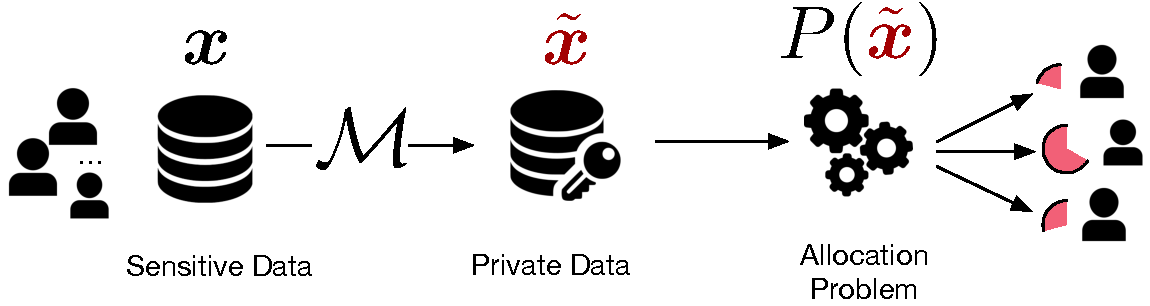
\includegraphics[width=0.9\columnwidth]{images/figure.pdf}
	\caption{Diagram of the private allocation problem.}
	\label{fig:framework}
\end{figure}
Figure \ref{fig:framework} provides an illustrative diagram.

Because random noise is added to the original dataset $\bm{x}$, the output $P_i(\tilde{\bm{x}})$ incurs some error. {\em The focus of this paper is to characterize and quantify the disparate impact of this error among the problem entities}. In particular, the paper focuses on two notations of errors.

\begin{definition}[Statistical bias]
	\label{def:bias}
	The statistical bias  $ B_P^i(\cM, \bm{x}) $ of the mechanism $\cM$ measures the difference between the expected private outcome with the true outcome:
	\begin{equation}
		\label{eq:bias}
		B_P^i(\cM, \bm{x}) =
		%\left|
		\EE_{\tilde{\bm{x}} \sim \cM(\bm{x})} \left[ P_i(\tilde{\bm{x}}) \right] - P_i (\bm{x}),
		%\right|,
	\end{equation}

\end{definition}

The paper also considers another notation of error which is the normalized version of the above bias.
\begin{definition}[Multiplicative error]
	The multiplicative error under mechanism $\cM$ and problem $P$ for entity $i$ is given by: $\nicefrac{B_P^i(\cM, \bm{x})}{P^i(x)}$

\end{definition}

Our notion of fairness will be based on these two notations of errors.


\begin{definition}[$\alpha$-fairness \cite{fioretto:CP-19}]
	Given the true data $\truedata$, the mechanism $\cM$ is said to be \emph{$\alpha$-fair} if, for any $i\in[n]$,
	\begin{equation*}
		\xi^{i}_P(\cM, \bm{x}) = ~\left\vert  B_P^i(\cM, \bm{x}) - B_P^j(\cM, \bm{x})
		\right\vert\leq \alpha\,,
	\end{equation*}
	where $ \xi^{i}_P(\cM, \bm{x})$ is referred to as the \emph{disparity error} associated with
	district $i$. The mechanism $\cM$ is \emph{$\alpha'$-minimally fair} if $\alpha'=\inf \alpha$ such that
	$\cM$ is $\alpha$-fair. To put it differently, the mechanism $\cM$ is \emph{$\alpha'$-minimally fair} if
	\begin{align*}
		\alpha'& = \max_{j\neq i}~\left\vert  B_P^i(\cM, \bm{x}) - B_P^j(\cM, \bm{x})
		\right\vert \\
		&= \max_{j\in [n]} B_P^j(\cM, \bm{x})   -\min_{j\in [n]}~ B_P^j(\cM, \bm{x}) \,.
	\end{align*}
\end{definition}
Throughout this report, every time we say that a mechanism is $\alpha$-fair, we mean that
it is $\alpha$-minimally fair.

% which characterizes the distance between the expected
% privacy-preserving allocation and the one based on the ground truth.
% The paper considers the absolute bias $|B_P^i|$, in place of the bias
% $B_P^i$, when $P$ is a decision rule. The distinction will become
% clear in the next sections.

	\section*{Problem Setting and Goals}
\label{sec:setting}
%%%%%%%%%%%%%%%%%%%%%%%%%%%%%%%%%%%%%%%%%%%%%%%%%%%%%%%%%%%%%%%%%%%%%


The paper considers a dataset $\bm{x} \!\in\! \cX \subseteq \RR^k$ of $n$ entities,
whose elements $x_i= (x_{i1},\ldots, x_{1k})$ describe $k$ measurable
quantities of entity $i \!\in\! [n]$, such as the number of individuals living
in a geographical region $i$ and their English proficiency.
The paper considers two classes of problems:
\begin{itemize}[leftmargin=*,labelsep=2pt,itemsep=0pt,parsep=2pt,topsep=2pt]
	\item An \emph{allotment problem} $P : \cX \times [n] \to \mathbb{R}$ is a function that distributes a finite set of resources to some problem entity. $P$ may represent, for instance, the amount of money allotted to a school district.
	\item A \emph{decision rule} $P: \cX \times [n] \to \{0,1\}$
	determines whether some entity qualifies for some benefits. For
	instance, $P$ may represent if election ballots should be described
	in a minority language for an electoral district.
% https://www.justice.gov/crt/about-language-minority-voting-rights
\end{itemize}
The paper assumes that $P$ has bounded range, and uses the shorthand
$P_i(\bm{x})$ to denote $P(\bm{x}, i)$ for entity $i$.
%
The focus of the paper is to study the effects of a DP data-release
mechanism $\cM$ to the outcomes of problem $P$. Mechanism $\cM$ is
applied to the dataset $\bm{x}$ to produce a privacy-preserving
counterpart $\tilde{\bm{x}}$ and the resulting private outcome
$P_i(\tilde{\bm{x}})$ is used to make some allocation decisions.

\begin{figure}[!t]
	\centering
	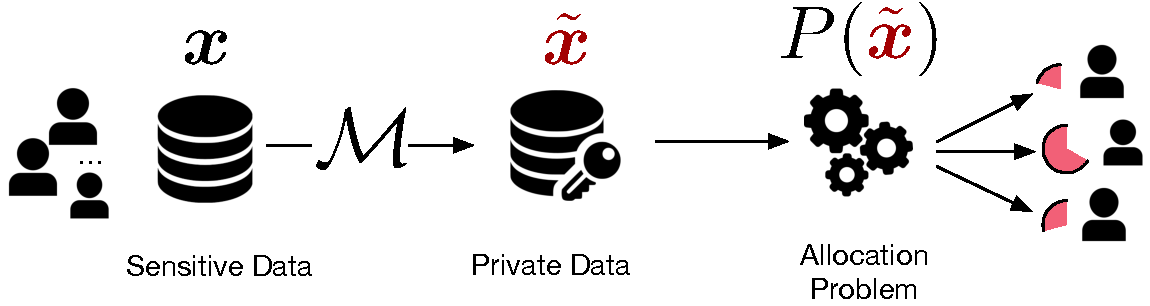
\includegraphics[width=0.9\columnwidth]{images/figure.pdf}
	\caption{Diagram of the private allocation problem.}
	\label{fig:framework}
\end{figure}
Figure \ref{fig:framework} provides an illustrative diagram.

Because random noise is added to the original dataset $\bm{x}$, the output $P_i(\tilde{\bm{x}})$ incurs some error. {\em The focus of this paper is to characterize and quantify the disparate impact of this error among the problem entities}. In particular, the paper focuses on two notations of errors.

\begin{definition}[Statistical bias]
	\label{def:bias}
	The statistical bias  $ B_P^i(\cM, \bm{x}) $ of the mechanism $\cM$ measures the difference between the expected private outcome with the true outcome:
	\begin{equation}
		\label{eq:bias}
		B_P^i(\cM, \bm{x}) =
		%\left|
		\EE_{\tilde{\bm{x}} \sim \cM(\bm{x})} \left[ P_i(\tilde{\bm{x}}) \right] - P_i (\bm{x}),
		%\right|,
	\end{equation}

\end{definition}

The paper also considers another notation of error which is the normalized version of the above bias.
\begin{definition}[Multiplicative error]
	The multiplicative error under mechanism $\cM$ and problem $P$ for entity $i$ is given by: $\nicefrac{B_P^i(\cM, \bm{x})}{P^i(x)}$

\end{definition}

Our notion of fairness will be based on these two notations of errors.

\begin{definition}[$\alpha$-fairness \cite{fioretto:CP-19}]
	Given the true data $\truedata$, the mechanism $\cM$ is said to be \emph{$\alpha$-fair} if, for any $i\in[n]$,
	\begin{equation*}
		\xi^{i}_P(\cM, \bm{x}) = ~\left\vert  B_P^i(\cM, \bm{x}) - B_P^j(\cM, \bm{x})
		\right\vert\leq \alpha\,,
	\end{equation*}
	where $ \xi^{i}_P(\cM, \bm{x})$ is referred to as the \emph{disparity error} associated with
	district $i$. The mechanism $\cM$ is \emph{$\alpha'$-minimally fair} if $\alpha'=\inf \alpha$ such that
	$\cM$ is $\alpha$-fair. To put it differently, the mechanism $\cM$ is \emph{$\alpha'$-minimally fair} if
	\begin{align*}
		\alpha'& = \max_{j\neq i}~\left\vert  B_P^i(\cM, \bm{x}) - B_P^j(\cM, \bm{x})
		\right\vert \\
		&= \max_{j\in [n]} B_P^j(\cM, \bm{x})   -\min_{j\in [n]}~ B_P^j(\cM, \bm{x}) \,.
	\end{align*}
\end{definition}
Throughout this report, every time we say that a mechanism is $\alpha$-fair, we mean that
it is $\alpha$-minimally fair.

% which characterizes the distance between the expected
% privacy-preserving allocation and the one based on the ground truth.
% The paper considers the absolute bias $|B_P^i|$, in place of the bias
% $B_P^i$, when $P$ is a decision rule. The distinction will become
% clear in the next sections.

%%%%%%%%%%%%%%%%%%%%%%%%%%%%%%%%%%%%%%%%%%%%%%%%%%%%%%%%%%%%%%%%%%%%%

	\section*{Title I School Funding Allocation}

\subsection{Allocation Problem}
The \emph{Title I of the Elementary and Secondary Education Act of
1965} \cite{Sonnenberg:16} distributes funds through its basic, concentration, and target grants which account for \$6.2B, \$1.3B, and \$4.2B of allocations, respectively. The federal allotment is divided among nearly 17000 qualifying school
districts in proportion to the count $x_i$ of children aged 5 to 17
who live in necessitous families in district $i$. Each grant is specified by a set of thresholds that determines which districts are eligible for that particular grant. We refer to \cite{Sonnenberg:16} which discusses the specifics of each grant, which we describe briefly here.

The basic allocation grant is formalized by:
\newcommand{\tfa}{P^F}
\newcommand{\rev}[1]{{\color{purple}{#1}}}
\newcommand{\add}[1]{{\color{darkgreen}{#1}}}
\newcommand*{\defeq}{\stackrel{\text{def}}{=}}
\def\aux{\mathrm{aux}}

\begin{align}
	\label{eq:allotment}%\tag{\text{$P_1$}}
	\tfa_i(\bm{x}) \defeq \left(
	\frac{x_i \cdot a_i}{\sum_{i \in [n] }x_i \cdot a_i}\right) \cdot F_{B}
\end{align}
where $\bm{x} = (x_i)_{i\in[n]}$ is the vector of all eligible districts counts
and $a_i$ is a weight factor reflecting students expenditures (defined as the adjusted state per-pupil expenditure). $F_{B}$ is the total basic Title I appropriation for the fiscal year. Finally, each funding grant is subject to different thresholds which define eligibility criteria for each district. This criteria is described in Table 1. The targeted grant is further weighted by population, as outlined in Section A of \cite{Sonnenberg:16}.

\begin{table}[t!]
	\centering
	\caption{Description of the thresholds that construct the eligibility criteria for each grant.}
	\begin{tabular}{lrr}
		\toprule
		Grant Type        & Eligibility Criteria            & Thresholds \\
		\midrule
		Basic Grant         & Population of eligible students & $>10$      \\
		& Proportion of eligible students & $>0.02$    \\
		Concentration Grant & District population             & $>6500$    \\
		& Proportion of eligible students & $>0.15$    \\
		Targeted Grant      & Population of eligible students & $>10$      \\
		& Proportion of eligible students & $>0.05$    \\
		\bottomrule
	\end{tabular}
	\medskip
	\raggedright
\end{table}

\subsection{Privacy Budget}
The Disclosure Avoidance System for the US Census Bureau defines a global rho that is distributed hierarchically.
The global privacy-loss budget for 2020 was defined as $\rho = 2.56$. The DAS suggests the use of this bound to conver
the $\rho$-based privacy-loss budgets to the $(\epsilon, \delta)$ equivalents.
$\epsilon = \rho + 2 * \sqrt{-\rho * \log_e{\delta}}$ where we define $\delta=10e-10$. In a 1-year estimate of the ACS,
there are $1426$ different "Detailed tables" available from the US Census Bureau. The rho allocation for the national,
state, and county level geographic hierarchies are $\frac{104}{4099}$, $\frac{1440}{4099}$, and $\frac{447}{4099}$
respectively. Assuming that the county level privacy-loss budget is split equally across these tables,
each field would have $\rho = 2.56 \cdot \frac{447}{4099} \cdot \frac{1}{1426} = 0.0001957 $ at the county level,
$\rho = 0.00063$ at the state level, and $\rho = 0.0000455$ at the national level.

We consider applying the Gaussian mechanism to satisfy differential privacy on children population estimate data along
with a hierarchical constraint that ensures that the sum of the noisy population estimate of sub-hierarchies are
consistent with their parent. For example, the sum of Title I-eligible children in the county-level subdivisions
of Illinois should be consistent with the noisy estimate of Title I-eligible children at the state level. We experiment
with three privacy budgets $\rho =  2.65$ and $\rho = 1.0$ and $\rho = 0.1$ to release privately the schools' population. These
private counts are used to determine amount of money each school district should receive using the allocation mechanisms
described above for the basic, concentration, and target grants. The statistical bias in Definition \ref{def:bias} here
represents the gain/loss in USD a school can have under the privacy preserving mechanism. \ref{fig:misalloc_total}
summarizes our findings of the bias as a function of district size for all $13,190$ districts. We observe that
misallocations are most pronounced at thresholds for each grant, and substantially impact smaller school districts more
than larger ones.

\begin{figure*}[h]
	\centering
	\begin{minipage}[b]{0.45\linewidth}
		\centering
		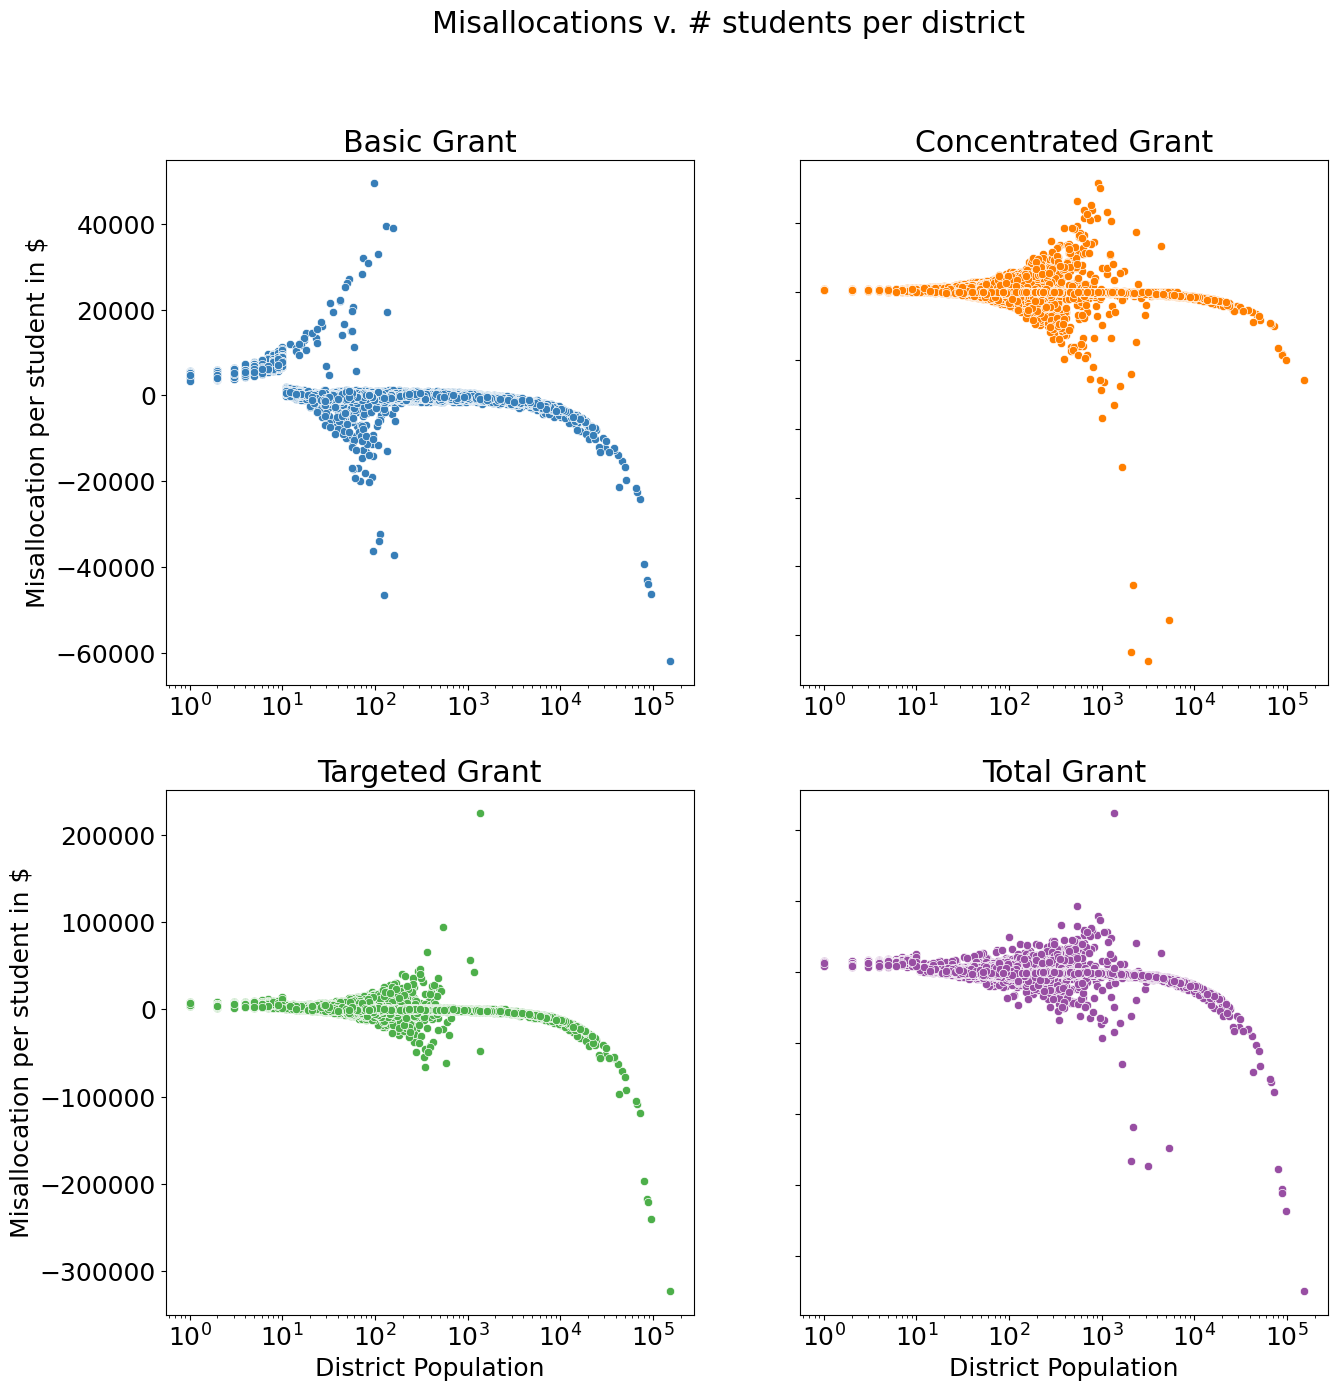
\includegraphics[width=\linewidth]{images/all_grant_errors_total}
		\caption{Misallocations in USD compared to district size}
		\label{fig:misalloc_total}
	\end{minipage}
	\hfill
	\begin{minipage}[b]{0.45\linewidth}
		\centering
		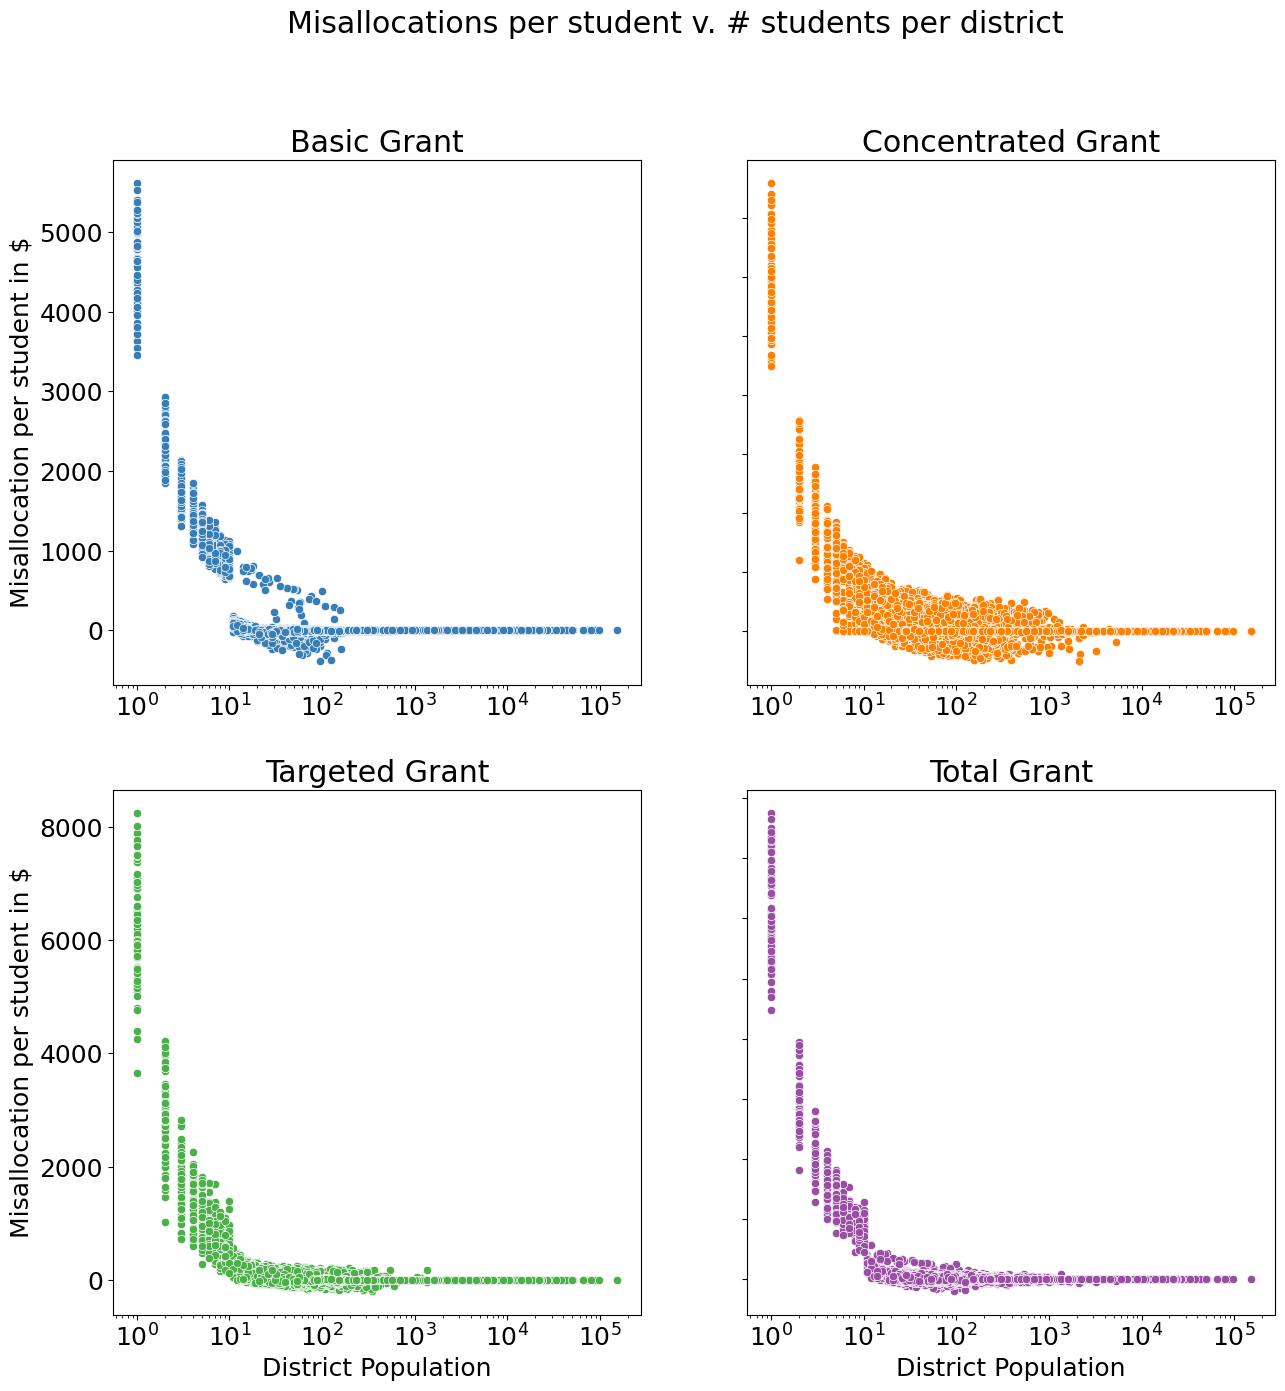
\includegraphics[width=\linewidth]{images/all_grant_errors_per_capita}
		\caption{Misallocations in USD per student compared to district size}
		\label{fig:misalloc_per_student}
	\end{minipage}
	\caption{We apply differential privacy with a privacy budget of $\rho=2.65$ to the population and eligible
	population counts of each district. We then plot the Title I misallocations for each district in the US for the
	basic, concentrated, and targeted grants, calculated using the allocation formulas outlined in \cite{Sonnenberg:16}.
	We observe that while large districts are more likely to receive larger misallocations, smaller districts are more
	likely to receive larger misallocations per student. We attribute these results to the complex interaction
	between differential privacy and the thresholds in the allocation formulas.}
	\label{fig:misalloc_comparison}
\end{figure*}


\begin{figure}[!ht]
	\centering
	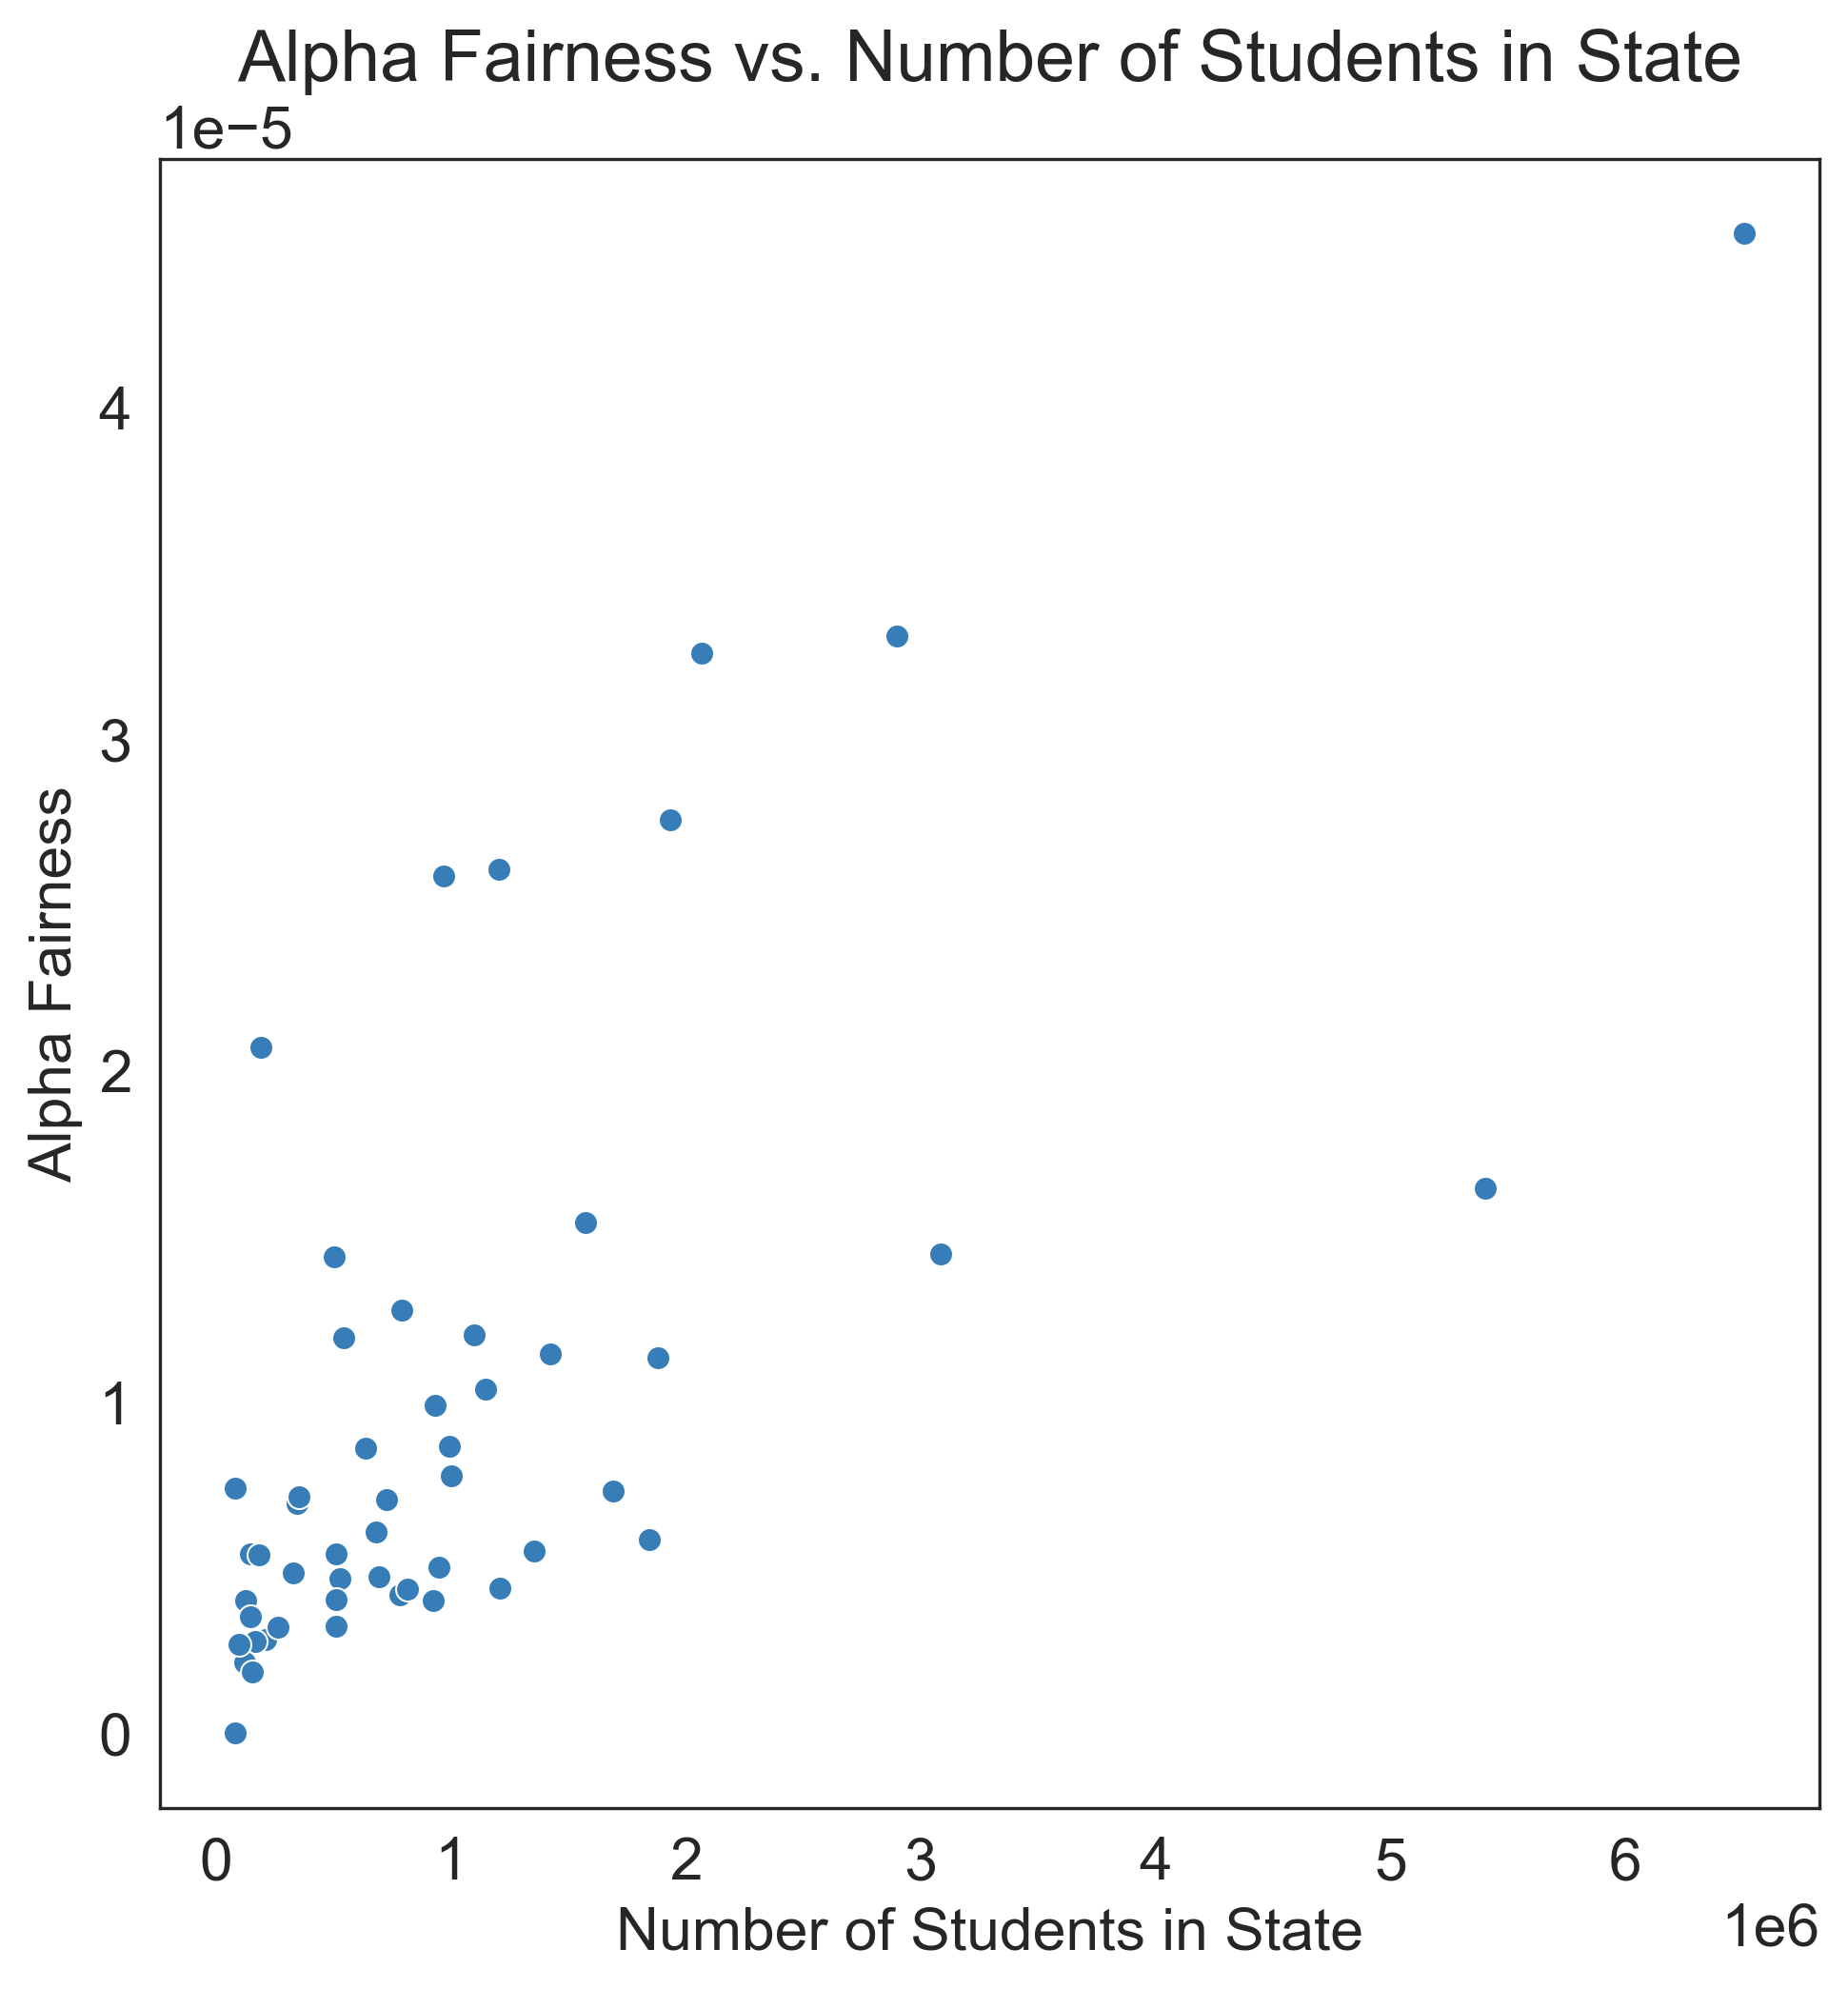
\includegraphics[width=0.6\linewidth]{images/af_vs_num_students_per_state}
	\caption{Correlation between number of students per state and alpha fairness at $\rho=2.65$}
	\label{fig:corr_fair_num_students}
\end{figure}


\begin{figure*}[h]
	\centering
	\begin{minipage}[b]{0.45\linewidth}
		\centering
		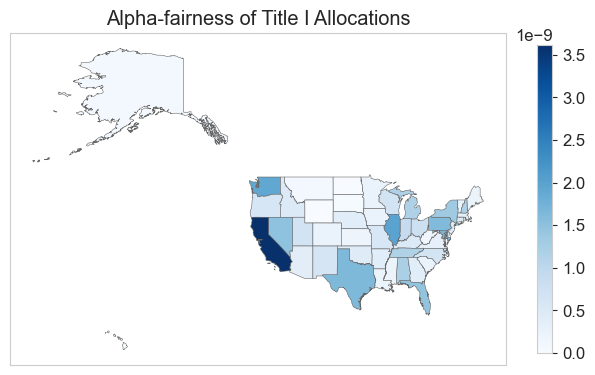
\includegraphics[width=\linewidth]{images/af_by_state.png}
		\caption{Level of $\alpha$ fairness per state under Baseline mechanism (BL) at $\rho = 2.56$}
		\label{fig:state_alpha}
	\end{minipage}
	\hfill
	\begin{minipage}[b]{0.45\linewidth}
		\centering
		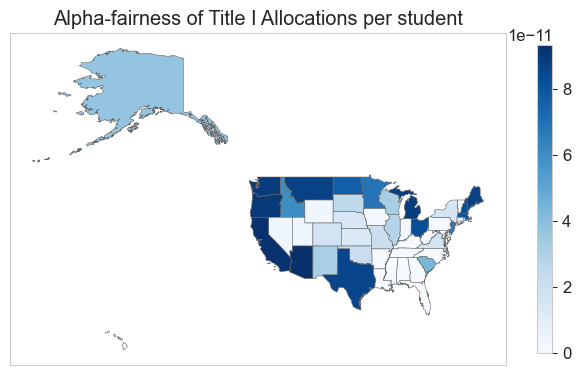
\includegraphics[width=\linewidth]{images/af_by_student.png}
		\caption{Level of $\alpha$ fairness per student under Baseline mechanism (BL) at $\rho = 2.56$}
		\label{fig:student_alpha}
	\end{minipage}
	\caption{Fairness comparison}
	\label{fig:fairness_comparison}
\end{figure*}



It can be seen from Figure \ref{fig:misalloc_total} that schools of low population receive far more money than they actually need
as a consequence of the bias in the allocation mechanism, while larger districts may actually receive less funding. This figure made a clear evidence on the disparate impact of the privacy preserving mechanism in practice.


\subsection*{Analysis}
In order to probe the effects of applying differential privacy to the Title I Allocation problem, we simulate
applying DP and recomputing grants for each district based on the distribution formula described by \cite{Sonnenberg
:16}. We compute 100K trials of samples to construct figures \ref{fig:misalloc_total} and the rest of our analysis.
We attribute the complex funding misallocation outcomes to the interaction of the several thresholds that consistute
each grant.

An in-depth analysis of the allocation of Title I education funds in districts requires an examination of both total
misallocations and misallocations per student. The consideration of these two perspectives is crucial for
understanding the impact of differential privacy on the distribution of funds and its implications for educational
equity.

Total misallocations offer a comprehensive overview by capturing the absolute magnitude of funding disparities across
states. By assessing the overall amount of misallocated funds, we can identify states that are disproportionately
affected. Such significant total misallocations can result in substantial disparities in educational resources,
thereby hindering the ability of disadvantaged districts to provide quality education. The findings from \ref{fig:misalloc_total},
which displays the data on total misallocations for each type of grant (basic, concentration, and targeted
), reaffirm this observation.

However, evaluating misallocations per student provides a more nuanced understanding of the fairness of funding
distribution. This perspective allows us to account for the relative impact on individual students within each state
. Misallocations per student highlight the distributional challenges faced by specific states and reveal the extent
to which educational inequalities are exacerbated. The data presented in Figure \ref{fig:misalloc_per_student}, whic
depicts misallocations per student, demonstrate that smaller districts tend to gain a substantial amount of funds
due to the application of differential privacy. In contrast, larger districts experience significant misallocations
without necessarily facing the same level of negative impact on a per-student basis.

It is important to recognize the specific implications of misallocations in different contexts. When funds are
misallocated in total, certain types of funding, such as specialized educational programs, additional resources, or
support services for at-risk students, may be inadequately supported. This can perpetuate existing disparities and
hinder efforts to address educational inequities, particularly in states with a higher population of disadvantaged
students. On the other hand, misallocations per student shed light on the deprivation of financial support
individual students require to succeed academically. This impacts the availability of crucial resources, including
instructional materials, qualified teachers, technology, and extracurricular activities, thereby impeding
educational progress and perpetuating systemic inequalities.

The correlation between a state's student population and the alpha fairness, as shown in
\ref{fig:corr_fair_num_students}, further supports the observed disparities. The positive Pearson correlation coefficient of
0.76 indicates that states with larger populations of students tend to have higher levels of alpha fairness,
indicating a greater degree of inequitable fund allocation.

Thus, the analysis of both total misallocations and misallocations per student provides a comprehensive understanding
of the impact of differential privacy on the allocation of Title I education funds. This dual perspective enables
policymakers to identify states disproportionately affected in terms of both the absolute amount of misallocated
funds and the relative impact on individual students. By gaining insights into the specific challenges faced by
different states, policymakers can devise targeted strategies to ensure a fair and equitable distribution of
education funds, taking into account the disparities arising from both large total misallocations in large districts
and smaller misallocations per student in small districts (Figure \ref{fig:misalloc_comparison}).

	\section*{Section 203 of the Voting Rights Act}

\begin{figure*}[h]
	\centering
	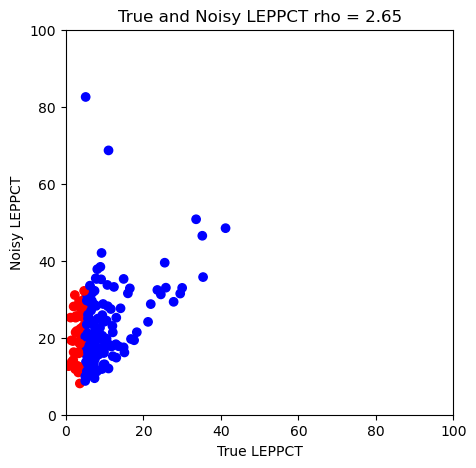
\includegraphics[width=0.5\linewidth]{images/true_noisy_leppct_2.65}
	\caption{LEPPCT vs. LEPPCT noisy values after DP mechanism at $\rho=2.65$}
	\label{fig:leppct}
\end{figure*}


Section 203 of the Voting Rights Act requires certain jurisdictions to provide bilingual election materials and
assistance to voters who are not proficient in English. To determine which jurisdictions are covered by this provision,
the Census Bureau collects data on the number and percentage of voting-age citizens who are members of a language
minority group and have limited English proficiency.

The Census Bureau uses three measures to calculate these numbers: the Limited English Proficient Population Count
(LEPPCT), the Illiteracy Rate (ILLRAT), and the Voting Age Citizen Language Minority Group Citizen Voting Age
Population (VACLEP).

The LEPPCT is the percentage of people in a language minority group who have limited English proficiency. The ILLRAT
is the rate of total LMG voting age citizens who are limited-English proficient and have less than a 5th grade
education. The VACLEP is the number of voting-age citizens who are members of a language minority group.

By using these three measures, the Census Bureau determines which jurisdictions meet the criteria for coverage under
Section 203. This information is then used by election officials to provide bilingual election materials and assistance
to voters who need it, ensuring that everyone has an equal opportunity to participate in the electoral process.

\subsection*{Allocation Formula}
Coverage from Section 203 is determined by a simple mechanism that ensures that a county satisfies the following conditions:

The ILLRAT is greater than the national illiteracy rate AND the LEPPCT is greater than 5\% OR the VACLEP is greater than
10,000. There are further nuances in this computation for American Indian and Alaska Native areas which we will refer
to \cite{Census203}.

\subsection*{Analysis}
In figure \ref{fig:leppct}, we observe the effects of applying differential privacy to the population counts in a similar
way to our approach in the Title I misallocations. We observe that applying DP noise can lead to false negative
outcomes, where communities that would originally receive coverage from Section 203 would be denied because their noisy
LEPPCT value would not satisfy the threshold constraints

	\section*{Differentially Private mechanisms}
To release privately the outcomes $P^F_i$ given a privacy constraint $\epsilon$, there are several mechanisms. These mechanisms can roughly be divided into the two categories, strict and non-strict allocation mechanisms. A strict allocation mechanism requires that
its outcome should always lie in the probability simplex $\Delta_n = \{x \  | x \in {\mathbb{R}^{+}}^{n}, \boldsymbol{1}^T x =1 \}$ while a non-strict allocation mechanism
only asks its output to be non-negative. The rest of this report aims to study the (approximate) optimal
(strict allocation) mechanisms under different fairness metrics.
\subsection*{Strict Allocation Mechanism}

\begin{definition}
	[Baseline Mechanism (BL)]
	The \emph{baseline mechanism} outputs the allocation for each distribute $i\in [n]$ as follows.
	\begin{equation*}
		\blmech{\noisydata}_i = \frac{a_i\cdot \relu{\tilde{x}_i}}{\sum_{j=1}^n a_j\cdot \relu{\tilde{x}_j}}\,.
	\end{equation*}
\end{definition}

Where $\tilde{x}_i$ is the noisy private population count, while the supscript $x_{+} = \max(x, 0)$ takes the non-negative part of the number $x$.


\begin{definition}
	[Projection onto Simplex Mechanism (PoS)]
	The \emph{projection onto simplex mechanism} outputs the allocation for each distribute $i\in [n]$ as follows.
	\begin{equation*}
		\posmech{\noisydata}_i = \underset{\bm{v}\in\RR^n}{\arg\min}~\norm{\bm{v}-\noisyalloc}_2\qquad\mathrm{s.t.}~
		\sum_{i=1}^n v_i = 1,~\bm{v}\geq \bm{0}\,.
	\end{equation*}
\end{definition}

\subsection*{Non-strict Allocation Mechanism}
\begin{definition}
	[Positive Allocation Mechanism (PA)]
	The \emph{positive allocation mechanism}
	outputs the allocation for each distribute $i\in [n]$ as follows.
	\begin{equation*}
		\pamech{\noisydata}_i  =  \relu{\nalloci{i}}= \relu{\frac{a_i\cdot \tilde{x}_i}{\sum_{j=1}^n a_j\cdot \tilde{x}_j}}\,.
	\end{equation*}
\end{definition}
\begin{definition}
	[Repair Mechanism (RP) \cite{pujol:20}]
	The \emph{repair mechanism} outputs the allocation for each distribute $i\in [n]$ as follows.
	\begin{equation*}
		\rpmech{\noisydata}_i  = \frac{a_i\cdot \relu{\tilde{x}_i}+\Delta}{\sum_{j=1}^n a_j\cdot \relu{\tilde{x}_j} - \Delta'}\,,
	\end{equation*}
	where
	\begin{equation*}
		\Delta= \frac{\ln\left(2n/\delta\right)}{\epsilon}\,,\qquad\Delta' =
		\frac{n\ln\left(2n^2/\delta\right)}{\epsilon}\,.
	\end{equation*}
\end{definition}

\begin{proposition}
	[No-penalty allocation \cite{pujol:20}]
	The following inequality holds with probability at least $1-\delta$.
	\begin{equation*}
		\rpmech{\noisydata}_i\geq \talloci{i}\,,\qquad\forall~i\in[n]\,.
	\end{equation*}
\end{proposition}


\section*{Source of unfairness}
We investigate the two main sources of unfairness highlighted in previous section: (1) shape of allocation function and (2) post-processing steps.
\subsection*{Shape of allocation function}

\begin{theorem}
	\label{lem:fair_bound_allottments}
	Let $P$ be an allotment problem which is at least twice differentiable.
	A data-release mechanism $\cM$ is $\alpha$-fair w.r.t.~$P$ for some
	$\alpha < \infty$ if there exist some constant values
% $c_i \; (i \in [n])$ such that,
% for all datasets $\bm{x} \in \cX$,
% \[
% \Tr(\bm{H}P_i)(\bm{x}) = c_i \;\; (i \in [n]).
% \]
	$c^i_{jl} \; (i \in [n], j,l \in [k])$ such that, for all datasets $\bm{x} \in \cX$,
	\[
		(\bm{H}P_i)_{j,l}(\bm{x}) = c^i_{j,l}   \;\; (i\in[n]\; j,l\in[k]).
	\]
\end{theorem}

\begin{corollary}
	\label{cor:2}
	If $P$ is a linear function, then $\cM$ is fair w.r.t.~$P$.
\end{corollary}


\begin{corollary}
	\label{cor:3}
	$\cM$ is fair w.r.t.~$P$ if there exists a constant $c$ such that,
	for all dataset $\bm{x}$,
	\[
		\mbox{Tr}(\bm{H}P_i)(\bm{x}) = c \;\; (i \in [n]).
	\]
\end{corollary}

\begin{corollary}
	Consider an allocation problem $P$. Mechanism $\cM$ is not fair
	w.r.t.~$P$ if there exist two entries $i, j \in [n]$ such that
	$\mbox{Tr}(\bm{H}P_i)(\bm{x}) \neq \mbox{Tr}(\bm{H}P_j)(\bm{x})$ for some dataset
	$\bm{x}$.
\end{corollary}

\noindent
The above implies that fairness cannot be achieved if $P$ is \emph{a
non-convex function}, as is the case for \emph{all} the allocation
problems considered in this paper. {\em A fundamental consequence of
this result is the recognition that adding Laplacian noise to the
inputs of the motivating example will necessarily introduce fairness
issues.} For instance, consider $\tfa$ and notice that the trace of
its Hessian
\[
	\mbox{Tr}(\bm{H}\tfa_i) = 2a_i \left[
		\frac{x_i \sum_{j\in[n]} a_j^2 - a_i \left(\sum_{j\in[n]} x_ja_j\right)}
		{\left(\sum_{j\in[n]}x_ja_j\right)^3}
		\right],
\]
is not constant with respect to its inputs. Thus, any two entries $i,
j$ whose $x_i \neq x_j$ imply $\mbox{Tr}(\bm{H}\tfa_i) \neq
\mbox{Tr}(\bm{H}\tfa_j)$. As illustrated in Figure \ref{fig:p1motivation},
Problem $\tfa$ can introduce significant disparity errors. For $\epsilon = 0.001,
0.01$, and $0.1$ the estimated fairness bounds are $0.003$, $3\times
10^{-5}$, and $1.2\times 10^{-6}$ respectively, which amount to an
average misallocation of \$43,281, \$4,328, and \$865.6 respectively.
The estimated fairness bounds were obtained by performing a linear
search over all $n$ school districts and selecting the maximal
$\mbox{Tr}(\bm{H}\tfa_i)$.


\subsection*{Impact of post-processing}
The post-processing steps can be applied at the inputs $x$, over the outcome $P^F_{i}(x)$ or at both. We investigate the impact of post-processing over input and outcome separately in this section.


\subsubsection*{Post-processing over the inputs}
This step is performed to make sure the released private counts satisfies consistency constraints \cite{cohen2021census}. For example, the released private counts should be non-negative integer numbers, or sum of counts at all cities' in a state should be equal to that state's count.


\noindent \textbf{Non-negative truncation} $\tilde{x} = \max(0, \tilde{x}) $

We have the following result which state that non-negative truncation introduces positive bias, and the closer to zero the true count is, the higher the bias.
\begin{theorem}
	\label{lem:exp_clipped_lap}
	Let $\tilde{x} = x + \mbox{Lap}(\lambda)$, with scale $\lambda > 0$,
	and $\hat{x} = \text{PP}^{\geq \ell}(\tilde{x})$, with $\ell < x$,
	be its post-processed value. Then,
	$$
	\EE[\hat{x}] = x + \frac{\lambda}{2} \exp(\frac{\ell - x}{\lambda} ).
	$$
\end{theorem}


\noindent \textbf{Integral transform}

The integral transform $\text{PP}^{\mathbb{N}}(z)$ is used when the released data should be of integral quantities. To make sure that this processing step does not introduce additional bias, we can rely on the stochastic rounding technique:

\begin{equation}
	\text{PP}^{\mathbb{N}}(z) = \begin{cases}
									\lfloor z \rfloor   \ \mbox{w.p.:} \  1 -(z- \lfloor z \rfloor ) \\
									\lfloor z \rfloor  +1 \ \ \mbox{w.p.:} \  z - \lfloor z \rfloor
	\end{cases}
\end{equation}


The stochastic rounding guarantees that $\mathbb{E} [\text{PP}^{\mathbb{N}}(\tilde{x})] = \tilde{x} $ so no additional bias will introduce to $\text{PP}^{\mathbb{N}}(\tilde{x})$


\subsubsection*{Post-processing over the outcomes}

\section*{Mitigating Solutions}
\subsection*{Mechanisms}
Different kind of post-processing mechanisms are considered in this section. These mechanisms
require that
their outcomes should always lie in the probability simplex $\Delta_n$. The rest of this work aims to study the (approximate) optimal mechanisms under different fairness metrics.
\begin{definition}
	[Baseline Mechanism (BL)]
	The \emph{baseline mechanism} outputs the allocation for each entity $i\in [n]$ as follows.
	\begin{equation*}
		\cM_{\mathrm{BL}}(\noisydata)_i = \frac{a_i\cdot \relu{\tilde{x}_i}}{\sum_{j=1}^n a_j\cdot \relu{\tilde{x}_j}}\,.
	\end{equation*}
\end{definition}

\begin{definition}
	[Projection onto Simplex Mechanism (PoS)]
	The \emph{projection onto simplex mechanism} outputs the allocation for each entity $i\in [n]$ as follows.
	\begin{equation*}
		\cM_{\mathrm{PoS}}(\noisydata)_i= \underset{\bm{v}\in\RR^n}{\arg\min}~\norm{\bm{v}-\noisyalloc}_2\qquad\mathrm{s.t.}~
		\sum_{i=1}^n v_i = 1,~\bm{v}\geq \bm{0}\,.
	\end{equation*}
\end{definition}




	\acknow{Please include your acknowledgments here, set in a single paragraph. Please do not include any acknowledgments in the Supporting Information, or anywhere else in the manuscript.}

	\showacknow{} % Display the acknowledgments section

	\bibsplit[2]

	% Bibliography
	\bibliography{lib}

\end{document}
